
\section{Power Control and Plant Simulation}
\label{sec:powercontrol}
\subsection{Introduction}
\label{sec:pwrintro}

Wind energy is very intermittent in its supply, and a method is needed for delivering power from an Energy Storage System (ESS) smoothly and efficiently.

Chemical plants typically operate in a steady state, which is why a simulation for this stop-start plant is very important.
Another important note to stress is that this plant is the sole energy provider for the location, so it is responsible for any shortfalls or surpluses in demand, and therefore potential damage to consumers.

In this chapter a means of providing a large population a reliable, safe power supply in an efficient manner is developed, as well as a simulation of the plant to perform validation on.

\subsection{Motivation}

Electrical grids are dynamic systems - loads change throughout the day, as do supplies.
A method for stabilising this system is beneficial to consumers as well as producers as significant deviations from the operating frequency ($\pm$4Hz) will cause generator meltdowns, damaged industrial equipment, and brownouts \cite{power:freqs}.
Typically power distribution grids work within a tighter tolerance of $\pm$0.05Hz to avoid possible grid failure \cite{power:freqs}, with Figure \ref{fig:freqgrid} showing typical regulation methods and consequences for grid frequencies.

Important to note is that the ESS has \emph{two} generation methods, the Solid Oxide Fuel Cell (SOFC) and the Ammonia Turbine.
Each of these devices have differing performances - the turbine boasts an impressive start-up time, whereas the SOFC boasts a significantly better thermal efficiency.
Clearly a method that offers a highly efficient (as well as stable) grid will reduce both initial and operating costs - as this will reduce the number of wind turbines required, ammonia to be generated, and thus reduce plant size.

Control methods explored include Linear Quadratic Regulator (LQR), Proportional Integral Differential (PID) and others to explore the best way to control the chemical plant. This section also touches on Model Predictive Control (MPC) - an approach that was employed in industry since the 1980s with initial applications in chemical plants and oil refineries.
The MPC is now commonplace in grid-balancing systems, as it offers optimal input, and takes account of constraints (such as maximum generation from a turbine). \cite{power:mpcadvs}

Classical control in the form of PID and LQR, while easier to implement, do not offer control over constraints, and therefore MPC is deemed a good candidate for the next iteration.
MPC was not implemented as full system dynamics (at this stage in the design process) are not yet known.

\subsection{Control Objectives}

Fundamentally the task objectives are separated into two main criteria:
\begin{itemize}
\item{Control Grid Frequency through supply and demand.}
\item{Regulate SOFC and Turbine inputs for the most cost-efficient control method.}
\end{itemize}
Most electrical grids ensure to keep net average frequency errors as zero for grid-based clocks to not run fast or slow. This report will not explore time-corrections. \cite{power:timecorrection}

\begin{figure}[htb]
\centering
        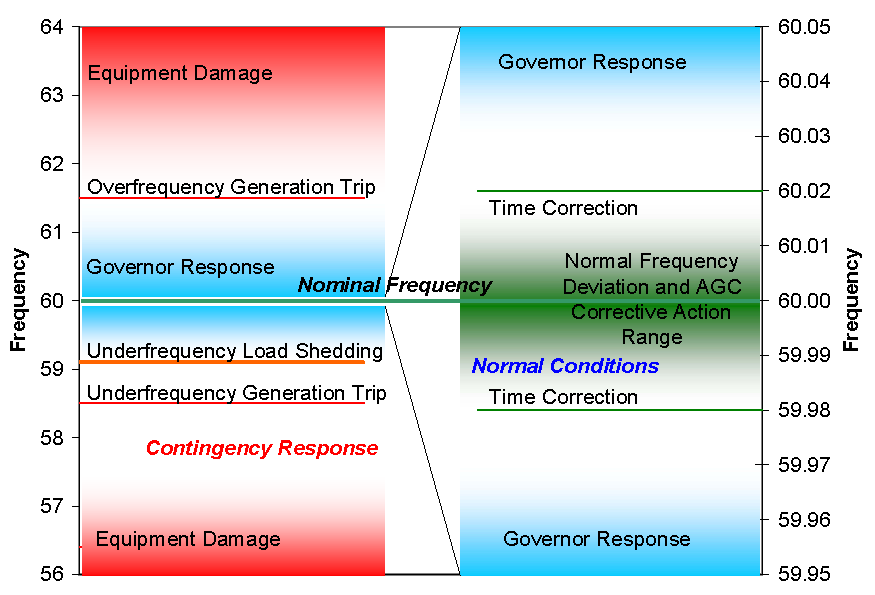
\includegraphics[scale=0.7]{images/freq.pdf}
\caption{Frequency tolerances for grid operation \cite{power:freqs}}
\label{fig:freqgrid}
\end{figure}
